\documentclass[journal,a4paper]{IEEEtran}
\usepackage{graphicx}
\usepackage{xcolor}
\usepackage{xeCJK}
%\usepackage{CJK}
\usepackage{fontspec}
\usepackage{geometry}
\usepackage{fancyhdr}
\usepackage{mdframed}
\usepackage{listings}
\usepackage{amsmath,amssymb,mathrsfs}
\usepackage{multirow}
\usepackage{float}
\usepackage{booktabs}
\usepackage{url}
\usepackage{hyperref}
\usepackage{array}
\usepackage{enumerate}
\usepackage{subfig}
\usepackage{longtable}

\bibliographystyle{IEEEtran}
\newtheorem{myDef}{\textbf{Definition}}
\newtheorem{myPro}{\textbf{Problem}}

\linespread{1.3}

\geometry{left=2.5cm,right=2.5cm,top=2.5cm,bottom=2.5cm}

\title{\huge{若干马氏链蒙特卡洛采样方法的比较与分析}}

\author{王禹~~无48~~2014011241}

\begin{document}

	\maketitle
	\begin{abstract}

		本文对估计受限玻尔兹曼机(RBM)的归一化常数经常使用的四种马氏蒙特卡洛抽样方法进行了复现改进,一定程度上提高了抽样方法的效率,并对这四种抽样方法的稳定性进行了比较分析。我使用MNIST手写数字数据库对四种方法进行了测试与比较,以此来对四种抽样方法的效率与性能进行评估与分析。

	\end{abstract}


	\section{Introduction}
	 手写体数字识别一直是一个研究热门问题,因为其应用广泛,且对识别的误识别率有着较高的要求。传统的分析方法是通过提取手写数字像素获得高维数特征集,再利用类似PCA等特征选择方法,筛选出维度较低的特征,在利用这些较低维度的特征训练神经网络,从而获得分类器。而本文所进行比较的四种方法,则均是直接将$ 28 \times 28 = 784$个像素点作为特征,输入到受限玻尔兹曼机(RBM)的观测变量端,并将该一层网络训练为分类器,训练过程中需要计算RBM的归一化常数。由于观测变量有784个,隐变量可以取任意数目,故最少共有$ 2^784 $种观测变量与隐变量的组合情况。这个数字对于计算机系统而言是巨大的,因此使用遍历方法计算归一化常数会有巨大的代价,所以需要使用合适的抽样方法对归一化常数进行逼近与估计。

	 本文所比较的四种采样方法分为三种。以AIS(Annealed Importance Sampling)\cite{salakhutdinov2009learning}为代表的方法采用的是构造了一个易于计算归一化常数的受限玻尔兹曼机RBM\_A,然后构造一系列从0到1的温度过渡因子,通过温度过渡,逐渐计算出目标受限玻尔兹曼机RBM\_B的归一化常数。以RTS(Rao-Blackwellized Tempered Sampling)\cite{carlson2016partition}和SAMS(Self-adjusted mixture sampling)\cite{tan2015optimally}为代表的方法,同样是构造了一个易于计算归一化常数的RBM\_A,也同样构造出了一系列由0到1的温度过渡因子。不同的是,其通过迭代将所有中间过程的归一化常数同时计算。经过足够多的次数后,归一化常数趋于稳定,而归一化常数数列的最后一项,即为目标RBM\_B的归一化常数。对于上述的两种方法,作者修改了部分迭代过程中的概率分布数学运算式,使得结果更快收敛。而TAP(Thouless-Anderson-Palmer)\cite{gabrie2015training}所采用的是则是将归一化常数的ln值,即自由能进行展开。因为无论是玻尔兹曼机还是受限玻尔兹曼机(RBM),都应当是系统能量最低的状态,即稳定状态。因此使用迭代法自由能的Legendre变换形式的最低状态所对应的参数后,将其带入总RBM自由能的展开式,进行一定的近似截取,即可获得总的自由能,即归一化常数的值。对于该种方法,笔者将其从原文献的二阶形式,精确到三阶迭代,获得了更加稳定的算法。
	\section{Model}
	本实验的基本模型为受限玻尔兹曼机(RBM),是深度学习的重要基础模型之一,其结构如图Fig.~\ref{fig1}所示:

		\begin{figure}[h]
		\centering
		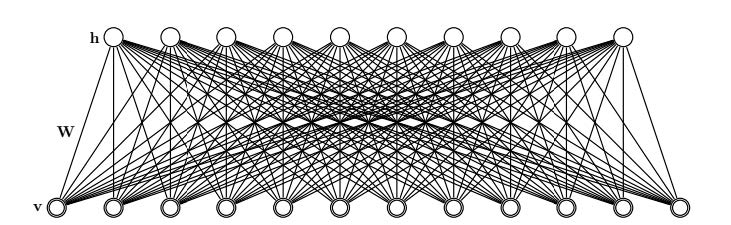
\includegraphics[width=0.5\textwidth]{1.jpg}
		\caption{RBM结构模型}
		\label{fig1}
		\end{figure}
	RBM由一层观测变量和一层隐变量构成,变量均为0,1取值。模型的能量符合物理中的玻尔兹曼分布,即:
		\begin{align}
		 & E(v,h;\theta) \notag \\
		 & =  -v^TWh-b^Tv-a^Th \notag \\
		 & =  -	\sum_{i}{\sum_j{ W_{ij}v_ih_j - \sum_i b_iv_i - \sum_j a_jh_j}}
		\end{align}
	而RBM模型观测变量和隐变量的联合分布为:
		\begin{align}
		p(v,h;\theta) = \frac{1}{Z(\theta)}e^{-E(v,h;\theta)}
		\end{align}
	其中,
		\begin{align}
		Z(\theta) = \sum_{v} \sum_h e^{-E(v,h;\theta)}
		\end{align}
	为归一化常数。

	\section{Methods}
	\subsection{Basic Method - MCMC}

	在叙述计算RBM归一化常数的采样方法之前,将先描述一般的MCMC(Markov Chain Monte Carlo)采样方法。
	\begin{myDef}
		为要模拟服从给定分布T的随机变量,用生成一个易于实现的不可约遍历链$ X=\{X_n,n\geq O\} $作为随机样本,使其平稳分布为$ \pi $的方法,称为马氏链蒙特卡罗方法.
	\end{myDef}
	而Metropolis-Hastings算法则为MCMC方法的一个改进,具体表述如下:

	\begin{table}[h]
	\centering
		\begin{tabular}{ll}
			\hline
			\multicolumn{2}{l}{\textbf{Algorithm 1:}Metropolis-Hastings Algorithm} \\
			\hline
			1: & 设$\pi = (\pi(i), i\in S)$为任意给定的概率分布,\\
			 & 而$ T = (T(i,j), i,j\in S)$为任选的易于实现 \\
			 & 的条概率转移矩阵\\
			2: & 给定$\pi = (X_n\in S, n\geq 0)$,由$T(X_n,·) $ \\
			 & 抽取Y,并计算\\
			 & $ \rho = min\{ 1,\pi(Y)T(Y,X_n)/(\pi(x)T(X_n,Y) \} $ \\
			3: & 抽取$ U \sim U[0,1]$,若$ U <\rho$, \\
			 & 则$ X_{n+1} = Y$,否则舍去Y,返回步骤2。\\
			\hline
		\end{tabular}
		\caption{Metropolis-Hastings Algorithm}
		\label{tab1}
	\end{table}

	使用上述算法可以有效的获得大量目标分布的抽样样本,具体的算法性能分析,请见下一小节。

	\subsection{RBM归一化参数与最似然概率估计}

	在详细描述四种具体的估计归一化常数的方法之前,需要首先说明一下抽样方法基于的模型。四种归一化参数的估计方法中,除了TAP外,都采用了相似的转移采样模型,具体模型如图Fig.~\ref{fig2}所示:
	\begin{figure}[h]
		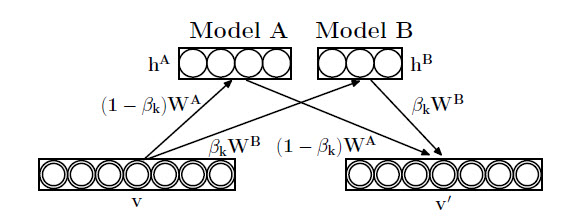
\includegraphics[width = 0.5\textwidth]{2.jpg}
		\caption{Transition Operation Model}
		\label{fig2}
	\end{figure}
	
	即构造一组$[0,1]$的温度过渡因子,从易于计算归一化常数($\beta = 0$)的RBM\_A,过渡到目标模型($\beta = 1$)RBM\_B。在某一个中间过程,即某一个特定温度因子$\beta$下,上述模型转移抽样应当如下数学表达式所示:
	\begin{flalign}
	p(h_j^A=1|\mathbf{v}) & = g\left((1-\beta_k)\left(\sum_i W_{ij}^A v_i +a_j^A\right)\right) \\
	\label{equ3}
%	\end{flalign}
%	\begin{equation}
	p(h_j^B=1|\mathbf{v}) & = g\left(\beta_k\left(\sum_i W_{ij}^B v_i +a_j^B\right)\right) \\
	\label{equ4}
	%\end{equation}
%	\begin{flalign}
	p(v_i'=1|\mathbf{h}) & = g((1-\beta_k)(\sum_i W_{ij}^A v_i + a_j^A) \\
	 & +\beta_k(\sum_i W_{ij}^B v_i +a_j^B))
    \label{equ5}
	\end{flalign}
	其中,$g(x)=\frac{1}{1+e^{-x}}$,为 深度学习模型中常用的logistic function。
	
	TAP算法虽然没有用到上述模型,但是仍然采用了恢复温度因子再做处理的的思想。

	\subsubsection{AIS\cite{salakhutdinov2009learning}}
		AIS 方法使用一系列过渡的$\beta_k$值,计算相邻两个状态之间的归一化常数的比值,通过比值的连乘,将归一化常数从易于计算的RBM\_A过渡到RBM\_B。本文实现的AIS具体算法如Table~\ref{tab2}所示:
		\begin{table}[h]
			\begin{tabular}{ll}
				\hline
				\multicolumn{2}{l}{\textbf{Algorithm 2:}Annealed Importance Sampling} \\
				\hline
				1: & 从$ 0=\beta_0<\beta_1<...<\beta_K=1$中随机选择一个$\beta_k$\\
				2: & 用选择的$\beta_k$采样一个$x_1$,满足最初的易于计算的\\
				 & RBM的$P_A$ \\
				3: & for $k = 1 : K-1$ do \\
				4: & ~~~~通过$T_k$转移矩阵,以及目前的$x_k$,采样$x_{k+1}$。\\
				5: & end for\\
				6: & 令$ \omega_k = \frac{Z_{k+1}}{Z_k} = \frac{P_{k+1}^*(x)}{P_{k+1}^*(x)}$,其中$ x \sim P_k$\\
				7: & $ Z_B = Z_A\prod_{k=1}^{K-1}\omega_k$,便可以获得最终结果\\

				\hline
			\end{tabular}
			\caption{AIS Algorithm}
			\label{tab2}
		\end{table}

		原始的算法中,$ \omega_k $ 一项表示成:$ \omega_k = \frac{Z_{k+1}}{Z_k} =\frac{1}{M} \sum_{i = 1}^{M} \frac{P_{k+1}^*(x^{(i)})}{P_{k+1}^*(x^{(i)})}$,$x^{(i)} \sim P_k$。即原始算法对每一种$\beta_k$值均作了M次抽样,之后将M次的结果作了平均。但是本算法中,将M取为1,也得到了较好的结果。
		而$P_k^*(\mathbf{v})$ 可以用如下的等式计算:
		\begin{align}
		 & P_k^*(\mathbf{v}) = e^{\beta_k\sum_i b_i^Bv_i} \left[\prod_{j=1}^{F_B} \left(1+e^{\beta_k(\sum_i W_{ij}^Bv_i+a_j^B)}\right)\right] \notag\\
		 & \times e^{(1-\beta_k)\sum_i b_i^Av_i} \left[\prod_{j=1}^{F_A} \left(1+e^{(1-\beta_k)(\sum_i W_{ij}^Av_i+a_j^A)}\right)\right]
		 \label{equ8}
		\end{align}

		具体的实验,实验结果以及分析见下一节。

	\subsubsection{TAP\cite{gabrie2015training}}
		由前述可知,RBM的联合分布为$P(v,h)=Z^{-1}e^{-E(v,h)}$,$Z$为归一化常数。取对数后,可得
		\begin{equation}
			\mathcal{L} = lnP(v) = - F^c(v)+F
		\end{equation}
		其中,$F = -\ln Z$为RBM的自由能,$F^c(v)= -\ln(\sum_he^{-E(v,h)})$为RBM的钳制自由能。本文关心重点为归一化常数的估计,即RBM的\textbf{自由能}。而吉布斯-波尔兹曼分布的\textbf{能量}在基于配置s的情况下应为$E(s) = -\sum_ia_is_i-\sum_{(i,j)}W_{ij}s_is_j$。
		为了降低计算\textbf{自由能}的计算量。首先恢复玻尔兹曼分布中的温度$\beta$对于基于玻尔兹曼分布的模型的影响,因为大多数模型中,将温度设定为常数1,从而忽略温度的影响。之后,将\textbf{能量}用外部辅助场$q$重写,可以得到$-\beta F[q] = ln \sum_se^{-\beta E(s)+ \beta\sum_iq_is_i} $ 而在经过Legendre变换,引入共轭变量$ m  = {m_i}$后,可以获得
		\begin{equation}
		 -\beta \Gamma[m]= -\beta \max_q[F[q]+\sum_iq_im_i]
		\end{equation}
		而\textbf{自由能}则为应该是经过Legendre变换后$q=0$的状态在经过反Legendre变换可得,即
		\begin{equation}
		 -\beta F= -\beta F[q=0] = -\beta \min_m[ \Gamma[m]] = -\beta  \Gamma[m^*]
		\end{equation}
		而对于任意的$A(\beta,m) \equiv -\beta\Gamma[m] $,展开后可得:
		\begin{align}
		A(\beta,m) & = A(0,m) + \beta \frac{\partial A(\beta,m)}{\partial\beta}\big|_{\beta=0} \notag \\
		& + \frac{\beta^2}{2}\frac{\partial^2A(\beta,m)}{\partial\beta^2}\big|_{\beta=0} + ...
		\end{align}
		因此可以得到:
		\begin{align}
		-\beta\Gamma(m)= &-\sum_i[m_i\ln m_i + (1-m_i)\ln(1-m_i)] \notag \\
		& +\beta \sum_i a_im_i + \beta \sum_{(i,j)} W_{ij}m_im_j \notag \\
		& +\frac{\beta^2}{2} \sum_{(i,j)} W_{ij}^2(m_i-m_i^2)(m_j -m_j^2) \notag \\
		& +\frac{2\beta^2}{3} \sum_{(i,j)} W_{ij}^3(m_i-m_i^2)(\frac{1}{2}-m_i) \notag \\
		& (m_j -m_j^2)(\frac{1}{2}-m_j) + ...
		\end{align}

		而回到RBM模型,我将其\textbf{能量}的Legendre变换由文献\cite{gabrie2015training}中的二阶推广的三阶形式,如下:
		\begin{align}
		\Gamma(m^v,m^h) \eqsim & -S(m^v,m^h) -\sum_i a_im_i^v  -\sum_i b_jm_j^h \notag \\
		& -\sum_{i,j} W_{ij}m_i^vm_j^h \notag \\
		& -\sum_{i,j} \frac{W_{ij}^2}{2}(m_i^v-(m_i^v)^2)(m_j^h -(m_j^h)^2) \notag \\
		& -\sum_{i,j} \frac{2}{3}  W_{ij}^3(m_i-m_i^2)(\frac{1}{2}-m_i) \notag \\
		& (m_j -m_j^2)(\frac{1}{2}-m_j) - ...
		\label{equ1}
		\end{align}
		这里将温度$\beta$设置为1,即我们所需要的RBM模型。上式精确到了三阶近似,若是只需要二阶近似,则把最后一项略去即可。
		而为了得到\textbf{自由能},需要式(\ref{equ1})能够取的最小值。因此需要$\frac{d\Gamma}{dm}=0$。因此可以通过如下经过推广的三阶迭代式,得到带入计算的$m^v,m^h$:
		\begin{flalign}
			m_j^h[t+1] & \leftarrow g[b_j+\sum_i W_{ij}m_i^v[t] \notag \\
			& - \sum_i W_{ij}^2\left(m_j^h[t]-\frac{1}{2}\right)(m_i^v[t]-m_i^v[t]^2) \notag \\
			& + \sum_i W_{ij}^3(m_i^v[t]-m_i^v[t]^2)(\frac{1}{2} - m_i^v[t]) \notag\\
			& (2(m_j^h[t]^2-m_j^h[t])+\frac{1}{3})] \\
			m_i^v[t+1] & \leftarrow g[a_i+\sum_j W_{ij}m_j^h[t+1] \notag \\
			& - \sum_j W_{ij}^2\left(m_i^v[t]-\frac{1}{2}\right)(m_j^h[t+1]-(m_j^h[t+1])^2)  \notag \\
			& + \sum_j W_{ij}^3(m_j^h[t+1]-m_j^h[t+1]^2)(\frac{1}{2}-m_j^h[t+1]) \notag\\
			& (2(m_i^v[t]^2-m_i^v[t])+\frac{1}{3})]
		\end{flalign}
		
	该$m^v,m^h$也为三阶近似项,若需要二阶近似,则将两式的最后一项舍去即可。
	
	\subsubsection{RTS\cite{carlson2016partition} and SAMS\cite{tan2015optimally}}
	RTS方法与SAMS方法比较类似,在此一并介绍。
	首先先介绍RTS方法。该方法也是构造出一系列温度过渡因子$ 0=\beta_1<\beta_2<...<\beta_K=1$与AIS一致。在某一温度因子情况下的中间过程,概率密度分布也与AIS一致,即
	\begin{equation}
		p(x|\beta_k)=\frac{f_k(x)}{Z_k}
	\end{equation}
	式中的$f_k(x)=P_A^*(x)^{1-\beta_k}P_B^*(x)^{\beta_k}$,其中$P_A^*,P_B^*$即如同式(\ref{equ8})中所示。
	式中的$Z_k$为温度处在$\beta_k$的情况下的归一化常数。
	RTS算法的核心便是通过多次迭代,同时更新所有温度过渡因子下的归一化常数。每次迭代的过程中,会同时对温度过渡因子$\beta$和观测变量$v$进行抽样。本算法中对观测变量的采样方法与本节开头的方法相同,即式(\ref{equ3}),(\ref{equ4}),(\ref{equ5})。这里主要叙述$\beta$的抽样方法。

	当$\beta \in \beta_k$是一个随机变量时,假定有一个先验概率$r(\beta_k)=r_k$,那么$x,\beta_k$的联合分布则如下表示:
	\begin{align}
	p(x,\beta_k) & = p(x|\beta_k)r_k, \\
	& = \frac{f_k(x)r_k}{Z_k}
	\end{align}
	由于$Z_k$是我们需要求的,并不知道,但我们可以定义$\hat{Z_k}$则
	\begin{equation}
	q(x,\beta_k) \propto \frac{f_k(x)r_k}{\hat{Z_k}}
	\end{equation}
	由于联合分布已经知道,文献\cite{carlson2016partition}定义出:
	\begin{equation}
	q(\beta_k|x) = \frac{f_k(x)r_k/\hat{Z_k}}{\sum_{l=1}^{K} f_l(x)r_l/\hat{Z_l}}
	\end{equation}
	有了上述的概率分布,我们便可以通过采样出的$x_k$,对下一次迭代使用的$\beta_s$进行抽样。具体来说,便是令$q(\beta_1),q(\beta_2),...,q(\beta_K)$依次按照其值,在$[0,1]$的轴上占据一定位置。取一符合$U(0,1)$的随机变量,该变量落入哪一个$q(\beta_k)$的区间,则将该$\beta_k$作为下一次迭代使用的$\beta$。而每次迭代中,则采用$ \hat{Z_k^{RTS}} = \hat{Z_k}\frac{r_1}{r_k}\frac{\hat{c_k}}{\hat{c_1}}$对归一化常数进行更新,其中$\hat{c_k}=\frac{1}{N} \sum_{i=1}^N q(\beta_k|x^{(i)})$。

	但是原始文章所采用的$q(\beta_k|x;\hat{Z_k})$收敛效果并不好,因此我将$q(\beta_k|x;\hat{Z_k})$定义时进行了改进。由文献\cite{salakhutdinov2009learning}中指出,对于任意一个$beta_k$,其未归一化的中间概率分布应当为式(\ref{equ8})所示。将其归一化之后,应当与$q(\beta_k|x;\hat{Z_k})$等价。而将$q(\beta_k|x;\hat{Z_k})$中的易于计算归一化常数的RBM的影响项从$q(\beta_k|x;\hat{Z_k})$中去除,即将$q(\beta_k|x;\hat{Z_k})$除以$Z_A^{1-\beta_k}$。经过这样的处理后,收敛效果得到了较好的提升。

	具体的算法步骤见下表TABLE~\ref{tab3}:
	\begin{table}[h]
		\begin{tabular}{ll}
			\hline
			\multicolumn{2}{l}{\textbf{Algorithm 3:}Rao-Blackwellized Tempered Sampling} \\
			\hline
			1: & 初始化$ 0=\beta_0<\beta_1<...<\beta_K=1$\\
			   & 初始化$\ln Z_k=0,k=2,...,K$ \\
			   & 初始化$\hat{c_k}=0,k=2,...,K$ \\
			2:& while $max{abs(\hat{c_k}-\frac{1}{K})}>Tlimit$\\
			3: & ~~~~for $i = 1 : N$ do \\
			4: & ~~~~~~~~通过转移矩阵(即式(\ref{equ3})(\ref{equ4})(\ref{equ5})),以及目前 \\
			   & ~~~~~~~~的$\beta_k$,采样$x$。\\
			5: & ~~~~~~~~通过$q(\beta_k|x;\hat{Z_k})$采样下一次迭代的$\beta$ \\
			6: & ~~~~~~~~更新$\hat{c_k} \leftarrow \hat{c_k} + \frac{1}{N} q(\beta_k|x)$ \\
			7: & ~~~~end for\\
			8: & ~~~~更新$\hat{Z_k}^{RTS} \leftarrow \hat{Z_k}\frac{r_1}{r_k} \frac{\hat{c_k}}{\hat{c_1}}$ \\
			9: & end while\\

			\hline
		\end{tabular}
		\caption{RTS Algorithm}
		\label{tab3}
	\end{table}

	而SAMS与RTS大体相似,算法步骤也基本相似,但是具体来说,根据文献\cite{tan2015optimally}所示,其更新$Z_k$的方法以及抽样$\beta$的方法不一样。这里先指出$\beta$的抽样方法不同之处。如上所示,RTS的$\beta$抽样方法,是全局抽样(global jump),即下一次抽样的$\beta_k$的位置可以是那组$\beta$的任意值,但是根据文献\cite{salakhutdinov2009learning}所示,SAMS的抽样方法是局部抽样(local jump),即每次抽取的下次的$\beta$值只能是本次$\beta$的相邻的$\beta$值。根据测试,global jump使得归一化参数更新速度过快,容易造成过冲,导致预估的归一化常数过大,此处使用local jump,能有效的控制收敛的速度在一个合适的范围。
	而SAMS的归一化常数更新的方法与RTS也不相同。RTS通过两层循环,先更新$\hat{c}$,再新$\hat{Z}$,从而实现归一化常数的估计。而SAMS的更新方法则如下描述:
	
	令$\zeta = \ln Z$,则:
	\begin{align}
		& \zeta^{(t-\frac{1}{2})} = \zeta^{(t-1)} + \notag \\ 
		& \lambda\{\frac{q_1(·;\hat{Z}^{(t-1)})}{r_1},\frac{q_2(·;\hat{Z}^{(t-1)})}{r_2},...,\frac{q_K(·;\hat{Z}^{(t-1)})}{r_K}\},
	\end{align}
	\begin{equation}
		\zeta^{(t)} = \zeta^{(t-\frac{1}{2})} - \zeta_1^{(t-\frac{1}{2})} \notag
	\end{equation}
	其中$\zeta_1^{(t-\frac{1}{2})}$为$\zeta^{(t-\frac{1}{2})}$的第一项,而$\lambda$满足如下的关系,以控制收敛的速度:
	
	$\lambda = \Big\{ \begin{matrix}
			\min(\pi_j,t^{-\beta}) & if~t \leq t_0 \\
			\min\{\pi_j,(t-t_0+t_0^{\beta})^{-1}\} & if~t > t_0 \\
			\end{matrix} $
	
	而此处的$q_k$仍采用了我在RTS中叙述过的改进,将RBM A的能量部分除去,以获得更好的收敛效果。
	
	\section{Analysis of Method \& Results}
	由于程序的运行时间和机器的配置有着较大的关系,本文的仿真实验,都是在CPU为i7-6700 @3.4GHz,内存16GB的电脑上运行的。
	\subsection{MCMC}
	为了验证MCMC,我们进行估计二维高斯的相关系数的实验。

	\begin{myPro}
		用 Metropolis-Hastings算法,对下述二维高斯分布进行随机采样
		\begin{equation*}
		\mathcal{N}\left\{\begin{pmatrix}x_1\\x_2\end{pmatrix}\bigg|\begin{pmatrix} 5 \\ 10 \end{pmatrix},\begin{pmatrix} 1 & 1\\1 & 4\end{pmatrix}\right\}
		\end{equation*}
		使用生成的随机样本来估计二维高斯函数的相关系数,并与真值比较。
	\end{myPro}

		由于这里抽样的采样点为一个二维向量,且在$\mathbb{R}^2$上式连续。因此T取有限大小会对转移产生误差。因此在本题中,没有构造出真实的转移矩阵T,而是假定转移矩阵T为一个所有元素都相同且符合马尔科夫转移性质的矩阵,即每一行相加为1。这种情况下,上述算法Table~\ref{tab1}中的$ T(Y,X_n) $与$T(X_n,Y)$相消,故只需要计算即将抽样的样本点的概率密度与前一个已经确认的样本点的概率密度作比值,在与一个在$ [0,1] $均匀分布的随机变量作比较后,来判断是否转移成功即可。而由于T为完全均匀的转移矩阵,因此下一个抽样点的抽取应当完全随机抽取。这里为了提高抽取的命中率,我将$x_1$与$x_2$分别按照独立的两个一维高斯分布抽取随机数,一维高斯分布的均值与标准差均来自于二维随机分布中的均值与协方差矩阵。同样,这样的抽样方法,也使得最终的结果的相关系数与抽样点的个数无关,不会随着抽样点的数目增加而变得更加接近真值。
		
		理论的相关系数真值应当为0.5。使用MATLAB仿真相关系数分布在$[0.484,0.497]$之间。
		为评判MCMC的准确性,多次重复独立试验,每次试验均抽取5万个采样点。讲这些实验所得的相关系数计算所得结果的方差,结果如下:
		\begin{center}
		\begin{tabular}{c|cc}
			\hline
			运行次数 & 相关系数均值 & 结果方差\\
			\hline
			5 & 4.912 & $5.49\times10^{-6}$ \\
			10 & 4.902 & $2.20\times10^{-5}$ \\
			20 & 4.899 & $3.69\times10^{-5}$ \\
			50 & 4.934 & $1.74\times10^{-5}$ \\
			100 & 4.923 & $1.67\times10^{-5}$ \\
			\hline
		\end{tabular}
		\end{center}
	
		首先分析本方法的准确性,由上述结果可见,多次运行本MCMC方法的方差非常小,为$10^{-5}$量级,而相关系数为$10^{-1}$量级。因此可以认为该MCMC抽样方法准确性相当高,几乎没有误差,同时,其抽样出的样本的相关系数与真值也非常接近,最大误差在0.1左右。
		
		其次是对算法效率的分析。运行一次生成5万个抽样点的MATLAB程序需要大概1s到2s的时间,主要时间开销在抽样主程序上。其次为了实现该算法,完成了一个计算二维正太分布概率密度的函数,该函数调用较为高效,3s的时间可以调用300万次。总体程序的效率较高。

	\subsection{AIS}
		在本实验实现AIS方法时,划分的温度过渡因子越细致,即$\beta$的集越大,所得到的结果越加精细,估计值更加贴近真值,但相对的运算的代价会变大,计算速度会变慢。具体的算法,在前述部分已经得到了讲解,在此对算法进行分析。
		
		首先分析程序运行效率。为了提高程序效率,令$ \omega_k = \frac{Z_{k+1}}{Z_k} =\frac{1}{M} \sum_{i = 1}^{M} \frac{P_{k+1}^*(x^{(i)})}{P_{k+1}^*(x^{(i)})}$中的$M=1$,既可以减少抽样次数,提高程序效率,也可以获得较好的结果。在尽可能获得准确的结果的情况下,令$\beta$的取值更加精细。根据实验结果来看,$\beta$的精细程度需要根据RBM的隐变量数目来动态决定。根据实验结果,对于10个隐变量取$\beta$数组的元素数为3万,20个隐变量模型的为30万,100,500个隐变量的模型均取为6万。而根据MATLAB本身的运算特性,尽可能的将所有的循环改写成为矩阵运算后,程序的运行效率得到了大大的提高。经过MATLAB仿真测试,h10的模型,运行时间为10s;h20的模型运行时间为60s;h100的模型运行时间为100s;h500的模型运行时间为264s。而该函数主要耗费效率的部分是抽样算法,抽出下一个观测变量的运算,以及一些求和运算,这些运算都无法避免或者使用矩阵乘法提高运算效率。
		
		再分析程序的准确性,将AIS函数循环20次,计算归一化常数的方差值,所得的结果如下表TABLE~和下图Fig.所示:
		\begin{center}
		\begin{tabular}{c|cc}
			\hline
			Model & Normalized Coef& Result Var \\
			\hline
			h10 & 225.89 & 0.1939 \\
			h20 & 218.23 & 19.4639 \\
			h100 & 348.5343 & 0.1089 \\
			h500 & 460.9204 & 0.0962\\
			\hline
		\end{tabular}
		\end{center}
		通过上述结果可以看出,除了h20的模型之外,AIS的结果是非常稳定的,每次产生的归一化常数的值也较为相似,方差非常小。而h20的结果方差较大,可能的原因在于训练模型时,获得参数结果不太好,导致了计算归一化常数的值得结果方差较大。可以看出,AIS算法除了花费的时间非常长之外,获得结果的准确性非常高。

	\subsection{TAP}
		而对TAP算法进行分析时,可以发现由于TAP算法是一种近似算法。近似造成其估计的归一化常数值与真值之间可能会存在一个恒定的误差,多次运行试验时得到的一组估计归一化常数的方差也非常小。根据原始公式,显然结果方差与与真值的误差会随着近似程度的增加,会逐渐变小。
		
		本文实现了TAP的二阶近似算法TAP2与三阶近似算法TAP3。两个算法的运行性能结果如下表所示:
		\begin{center}
		\begin{tabular}{c|ccc}
			\hline
			Model & TAP2 Var & TAP3 Var & Norm Coef\\
			\hline
			h10 & 0.0213 & 0.0001 & 207.2 \\
			h20 & 1.0136 & 0.0001 & 221.1 \\
			h100 & $7.35\times 10^{-11}$ & 0.0036 & 335.7857 \\
			h500 & $1.04\times 10^{-4}$ & 0.0002 & 432.6158 \\
			\hline
		\end{tabular}
	\end{center}
		通过上述结果可以发现,TAP算法获得的归一化常数与真值之间有一定误差,但是每一次TAP得到的结果的方差较小,因此TAP算法是一个稳定的算法,但是得到的结果偏差较远。TAP算法的时间开销较小,每次调用的时间都在1s以内,这和他不需要逐步提高温度因子来逼近最终结果的玻尔兹曼机有关。通过快速迭代,TAP可以较快的得到结果下图Fig.\ref{fig4}为重复试验调用TAP3函数50次时,每次的结果图,Fig.\ref{fig5}为一次调用TAP3中,其当前自由能能量与上次自由能能量之差的结果。通过该图可以发现,TAP3算法能够以较快的速度收敛,但是估计出的归一化常数,与真实值有着一定的差距。
		\begin{figure}[h]
			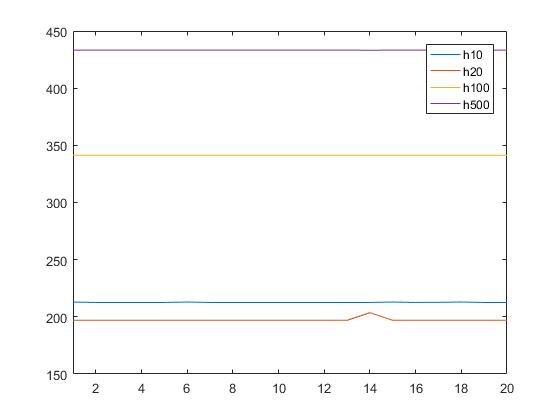
\includegraphics[width=0.5\textwidth]{4.jpg}
			\caption{重复试验50次结果}
			\label{fig4}
		\end{figure}
		\begin{figure}[h]
			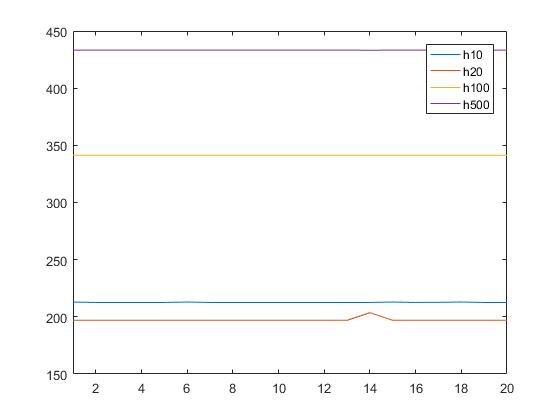
\includegraphics[width=0.5\textwidth]{4.jpg}
			\caption{TAP3收敛效果}
			\label{fig5}
		\end{figure}
	
	\subsection{RTS}
		RTS的结果收敛性较差,波动性也较高。这个和RTS算法中的易于计算归一化常数的RBM参数设置有关。最开始,作者尝试使用全为0的参数设置为RBM A的参数。然而,这种情况下RTS算法并不收敛,其估算出的误差呈现周期性的波动。因此,我尝试改变RBM A的一个或两个参数。由文献\cite{salakhutdinov2009learning}中指出,当$W_A$取为全0矩阵时,有$P^A(\mathbf{v})=\prod_ip_A(v_i)=\prod\frac{1}{1+e^{-b_i}}$。由此可以解出$b_i = \ln \frac{P_i^A}{1-P_i^A}$。因此,在此将$b^A$设定为如下的值。令$b^A=\ln \frac{f}{1-f}$,其中$f$为$1\times784$的向量,其计算方法如下所述。读取训练RBM参数的训练集,应当为$N\times784$的数据集,统计784个变量的N组数据中1出现的频率,即为所需要的$f$。而为避免出现$\inf$与$-\inf$的情况,可以将784个1的频数都增加一个较小的值如5。通过该方法,获得不含有$\inf$与$-\inf$的$b^A$。将其带入运算后,收敛性得到了较好的提高。
		以h10为例,其收敛速度如下图Fig. ~\ref{fig6}所示
		
		\begin{figure}[h]
			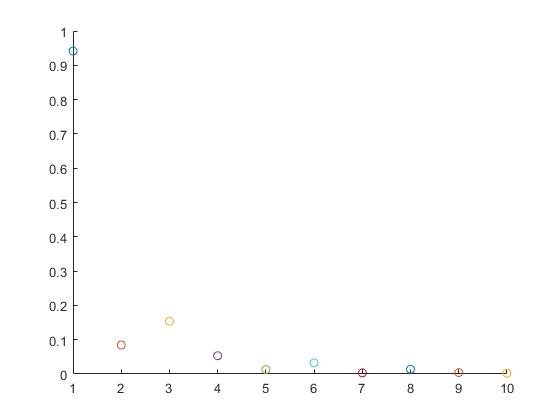
\includegraphics[width = 0.5\textwidth]{6.jpg}
			\caption{h10模型收敛速度}
			\label{fig6}
		\end{figure}
	
		RTS的运行性能如下表所示:
		\begin{center}
		\begin{tabular}{c|cc}
	\hline
	Model & RTS Var & Norm Coef \\
	\hline
	h10 & 0.2963 & 226.1005\\
	h20 & 2.1839 & 220.6264\\
	h100 & 12.3514 & 347.7237\\
	h500 & 0.2188 & 463.1204\\
	\hline
\end{tabular}
		\end{center}
		
		仿真过程中发现,若不能快速达到收敛条件,RTS容易陷入循环中,最终使得算法的时间开销较长,因此设置合适的阈值与RBM\_A的参数,对于RTS得到快速正确的结果非常的重要。而综合来看,因为作者本人没有花费足够的时间去寻找所有合适的参数,因此对于隐变量数目较少的模型,收敛效果较好,对于隐变量数目较多的模型,最后难以收敛。但是一旦能够成功地脱离循环,得到最终的归一化结果,可以发现,RTS迭代得到的结果距离真值精确程度与AIS一致。因此对于RTS算法而言,设计合适的阈值与迭代参数是最为重要的设计部分。
		
	\subsection{SAMS}
		SAMS的估计结果相较AIS偏离不远,且其运行速度比AIS要快,收敛性也比RTS要好。因此也是一种比较优质的估计归一化参数的方法。
		SAMS算法的结果如下表所示:
		\begin{center}
		\begin{tabular}{c|cc}
			\hline
			Model & SAMS Var & Norm Coef\\
			\hline
			h10 & 0.7467 &   226.45 \\
			h20 & 0.2188 & 210.17 \\
			h100 & 301.54 & 329.79\\
			h500 & 486.2 & 512.70\\
			\hline
		\end{tabular}
	\end{center}
		通过上述结果可以发现,SAMS的结果相对而言也比较稳定。与真值的误差随着隐变量的个数增加而变大。SAMS时间开销较小,h500的模型在30s内可以计算完成。但是,随着隐变量数量快速增加,SAMS的准确性也会随之降低,方差也随之增加,算法的稳定性下降,此时应当使用新的参数进行。
		
		而经过上述四个算法得到了归一化常数之后,我们可以对实验样本进行似然值的估计。似然值估计的方法,通过下式进行:
		\begin{align}
		P(v,\theta) & = \frac{1}{Z(\theta)}\sum_h e^{-E(v,h;\theta)} \notag \\
		& = \frac{1}{Z(\theta)} e^{b^{\top}v} \prod_{j=1}^F \left(1+e^{a_j+\sum_{i=1}^{D}W_{ij}v_i}\right)
		\end{align}
		通过该表达式,可以将总似然值计算得出。对于每一个测试集,$\frac{1}{Z(\theta)}$后面的部分是恒定的,只有归一化常数会对最后的结果产生影响。而最似然估计值越大,意味着测试集与模型匹配的越好。
		
	\section{Conclusion}
		综上所述,所有采样方法中,AIS方法为精确度最高的方法,但是其时间复杂度太高,且随着模型隐变量数目的增加而增长,若需要精确地估计归一化常数,则使用此方法较为合适。而RTS方法是收敛性最差的算法,需要对初始的参数做精巧的设计,才有可能使得RTS方法以较快的速度收敛。TAP方法为所有方法中速度最快的方法,低时间复杂度的代价便是归一化常数估计值与真值之间的误差较大。若对归一化常数不需要较为精确地结果,且需要处理大量的模型数据,使用此方法较为合适。而SAMS的相对于前述的三种算法而言,获得了折中的结果,即速度相比AIS获得了较大的提高,结果相对于TAP更为准确,而且易于收敛。该方法适合用于快速对归一化参数进行近似的估计。
		
	\section{Acknowledgement}
	感谢随机过程课程的欧智坚老师与戴音培助教对我学习过程中的困惑的解释。

	感谢无47班余东翰同学,无48班黄佳新同学,无48班徐瑞同学等对我学习RBM归一化参数的估计算法的帮助!

	\bibliography{IEEEabrv,bibfile}

\end{document}
